
	\documentclass{article}
	\usepackage{amsmath,amssymb}
	\usepackage[inline]{enumitem}
	\usepackage{blindtext}
	\usepackage{booktabs}
	\usepackage{graphicx}
	\usepackage{xcolor}
	\usepackage[vmargin = 1.5in, top = 1in, bottom = 1.2in, letterpaper]{geometry}
	\usepackage{listings}
	\usepackage{courier}
	\lstset{
	basicstyle = \small\tt,
	keywordstyle = \tt\color{blue},
	commentstyle = \it\color[cmyk]{1,0,1,0},
	stringstyle = \tt\color[RGB]{128,0,0},
	%frame = single,
	backgroundcolor = \color[RGB]{245,245,244},
	breaklines,
	extendedchars = false,
	xleftmargin = 2em,
	xrightmargin = 2em,
	aboveskip = 1em,
	tabsize = 4,
	showspaces = false
	}
	\begin{document}
	
	% \newfontfamily\courier{Courier New}

	
	\title{STAT 500 Homework 3}
	\author{Yifan Zhu}
	\maketitle
	
	\begin{enumerate}[leftmargin = 0 em, label = \arabic*., font = \bfseries]
	\item
	\begin{enumerate}
		\item \begin{enumerate*}[label = (\roman*)]
			\item Each sample is i.i.d. \item Samples are independent.
		\end{enumerate*}

		\item Each sample is normally distributed.
		\item Samples have the same variance. $\sigma_1 = \sigma_2 = \sigma$.

		\item 
		\begin{enumerate}[label = (\roman*)]
		\item The linear combination of normally distributed random variables is also normally distributed, and  $Y_1, Y_2, \cdots, Y_n$ are independent, so 
			\[E(\sum_{i = 1}^n Y_i) = \sum_{i=1}^n E(Y_i) = n \mu,\, Var(\sum_{i=1}^n Y_i) = \sum_{i=1}^n Var(Y_i) = n \sigma^2\]
			Thus $\sum_{i=1}^n Y_i \sim Normal(n \mu, n \sigma^2)$

			\item $\bar{Y} = \frac{1}{n}\sum_{i = 1}^n Y_i$ is a linear combination of normally distributed random variables. And
			\[E(\bar{Y}) = E(\frac{1}{n}\sum_{i=1}^n Y_i) = \frac{1}{n} n \mu = \mu,\, Var(\bar{Y}) = Var(\frac{1}{n} \sum_{i=1}^n Y_i) = \frac{1}{n^2} n \sigma^2 = \frac{\sigma^2}{n}\]
			Thus $\bar{Y} \sim Normal(\mu, \frac{\sigma^2}{n})$
			

		\end{enumerate}	
	
	\end{enumerate}

\newpage
	\item \begin{enumerate}
		\item  Summary statistics for the two sample distributions and boxplots.

		\begin{center}
	\begin{tabular}{ccccccc}
	\toprule
group&N&Mean&Std Dev&Std Err&Minimum&Maximum\\
\midrule 
Died&24&0.7279&0.0235&0.00481&0.6590&0.7650\\
Survive&35&0.7380&0.0198&0.00335&0.6870&0.7800\\
Diff (1-2)&&&&-0.0101&0.0214&0.00567\\
\bottomrule		

	\end{tabular}

\

\

	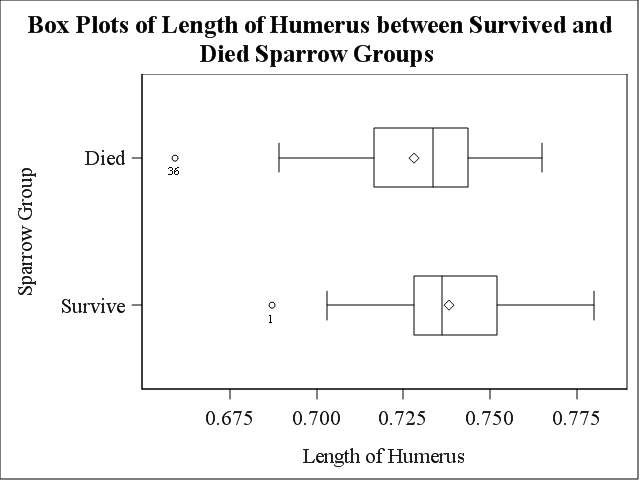
\includegraphics[width = 0.8\textwidth]{sparrowboxplot.png}
	\end{center}
From the summary statistic, the mean and the standard deviation of length of humerus of these two groups are similar. From the boxplot, we can see the IQR's are also similar. They overlap a lot, but the survived group seems to have longer humerus.

\item
Denote the mean length of died group $\mu_1$ and $\mu_2$ for the survived group. 

Null hypothesis $H_0$: $\mu_1 = \mu_2$.

Alternative hypothesis $H_a$: $\mu_1 \neq \mu_2$.

The standard deviations are similar, so we use the t-test with pooled standard deviation.

Obeserved test statistic $T = -1.78$

p-value: 8.09\%

The p-value is greater than $\alpha = 5\%$, so we accept the null hypothesis.

\item
$ \bar{Y}_1 - \bar{Y}_2 - t_{n_1 + n_2 -2, 1 - \alpha/2} S_p \sqrt{\frac{1}{n_1}+ \frac{1}{n_2}}= -0.0214,\, \bar{Y}_1 - \bar{Y}_2 + t_{n_1 + n_2 -2, 1 - \alpha/2} S_p \sqrt{\frac{1}{n_1}+ \frac{1}{n_2}}=0.00128$. Then $CI = (-0.0214, 0.00128)$.

Interpretation: we are 95\% confident that the difference of the mean length of humerus between the died sparrow and the survived sparrow ($\mu_1 - \mu_2$) is between -0.0214 and 0.00128.

\item

According to the analyses above, there is no significant difference between the means of died and survived sparrows. Thus we can conclude that he length of the humerus (arm bone) was not related
to whether or not the sparrow survived their injuries. 



	\end{enumerate}
	\newpage
\item 
\begin{enumerate}
	\item \ 

\begin{center}
\begin{tabular}{ccc}
\toprule
$n_1$ & $n_2$ & $Var(\bar{Y}_1 - \bar{Y}_2)$\\
\midrule
1 & 49 & $1.020 \sigma^2$\\
5 & 45 & $0.222 \sigma^2$\\
10&40&$0.125 \sigma^2$\\
20&30&$0.083 \sigma^2$\\
25&25&$0.080 \sigma^2$\\
30&20&$0.083 \sigma^2$\\
40&10&$0.125 \sigma^2$\\
45&5&$0.222 \sigma^2$\\
49&1&$1.020 \sigma^2$\\
\bottomrule
\end{tabular}
\end{center}

\item Equally divide them into $n_1 = 25$ and $n_2 = 25$. 

\item In Cauchy-Schuwarz Inequality
\[\sqrt{a_1^2 + a_2^2} \sqrt{b_1^2 + b_2^2} \geq \left|a_1 b_1 + a_2 b_2\right|\],
let $a_1 = \frac{\sigma_1}{\sqrt{n_1}},\, a_2 = \frac{\sigma_2}{\sqrt{n_2}},\, b_1 = \sqrt{n_1},\, b_2 = \sqrt{n_2}$. Then we have
\[\sqrt{\frac{\sigma_1^2}{n_1} + \frac{\sigma_2^2}{n_2}} \sqrt{n_1 + n_2} \geq \sigma_1 + \sigma_2 \Rightarrow \frac{\sigma_1^2}{n_1} + \frac{\sigma_2^2}{n_2} \geq \frac{(\sigma_1 + \sigma_2)^2}{n_1 + n_2}\]
equality holds if and only if when $\frac{\sigma_1 / \sqrt{n_1}}{\sqrt{n_1}} = \frac{\sigma_2 / \sqrt{n_2}}{\sqrt{n_2}} \Rightarrow \frac{\sigma_1}{n_1} = \frac{\sigma_2}{n_2}$. 

Hense, in order to have the least variance, we need to set $n_1 = \frac{50 \sigma_1}{\sigma_1 + \sigma_2},\, n_2 = \frac{50 \sigma_2}{\sigma_1 + \sigma_2}$.

	\end{enumerate}
\newpage
	\item
	\begin{enumerate}
		\item 
	Denote the mean of control group and therapy group $\mu_1$ and $\mu_2$. $T$ is the test statistic for t-test.

	Null hypothesis $H_0$: $\mu_1 = \mu_2$.

	Alternative hypothesis $H_a$: $\mu_1 \neq \mu_2$.

	Obeserved test statistic $\bar{Y}_1 - \bar{Y}_2 = -19.4706$.

	p-value: 1.79\%

	Decision: reject null hypothesis.

	Conclusion: The survival times for patients taking therapy and patients in the control group are different. Thus the therapy will make a difference in the survival time of patients for breast cancer.
	

	
	\item 
	Denote the mean of control group and therapy group $\mu_1$ and $\mu_2$. Sample mean of control group is denoted $\bar{Y}_1$ and sample mean of therapy group $\bar{Y}_2$. Because the sample standard deviations of these two group have a significant difference, we also need to considering using the Satterthwaite t-test. 

	Null hypothesis $H_0$: $\mu_1 = \mu_2$.

	Alternative hypothesis $H_a$: $\mu_1 \neq \mu_2$.

	Obeserved test statistic $T$ (pooled): -2.40

	p-value (pooled): 1.95\%

	Obeserved test statistic $T$ (Satterthwaite): -2.79

	p-value (Satterthewaite): 0.81\%

	Decision: reject null hypothesis.

	Conclusion: The survival times for patients taking therapy and patients in the control group are different. Thus the therapy will make a difference in the survival time of patients for breast cancer.

	\item The pooled t-test p-value and the randomization test p-value are similar, and the Satterthwaite t-test p-value is smaller than the randomization test p-value. Acctually they are all small enough to reject the null hypothesis and then to draw the same conclusion. But if we set the level $\alpha$ extreamly small, for example, in this case, $\alpha = 1\%$. Then when we adopt the Satterthewaite t-test p-value, we will reject $H_0$ and we will accept $H_0$ when we adopt the pooled t-test p-value and randomization test p-value.

\item

CI (pooled): $(-35.6941, -3.2470)$

CI (Satterthwaite): $(-33.5891, -5.3521)$

Interpretation (pooled): we are 95\% confident that survival time of the patients for breast cancer with therapy is between 3.2470 and 35.6841 months longer than the survival time of patients without therapy (control group).

Interpretation (Satterthwaite): we are 95\% confident that survival time of the patients for breast cancer with therapy is between 5.3521 and 33.5891 months longer than the survival time of patients without therapy (control group).
 	\end{enumerate}

\end{enumerate}
	
	
	
	\end{document}